\documentclass[12pt, a4paper]{article}

\usepackage[utf8x]{inputenc}
\usepackage[greek, english]{babel}
\usepackage{caption}
\usepackage[section]{placeins}
\usepackage{balance}
\usepackage{dblfloatfix}
\usepackage{hyperref}
\usepackage{color}
\usepackage{graphicx}
\usepackage{float}

%\usepackage[margin=2cm]{geometry}
%\usepackage{graphicx,wrapfig,lipsum}

\newcommand{\en}{\selectlanguage{english}}
\newcommand{\gr}{\selectlanguage{greek}}

\hypersetup{
	colorlinks=true,
	linkcolor=blue,
	filecolor=magenta,
	urlcolor=blue,
}

\begin{document}
	
\gr
\begin{titlepage}
	
	\begin{center}
		\vspace*{0.5cm}
		
		\LARGE
		\textbf{\gr ΠΜΣ ΕΠΙΣΤΗΜΗ ΚΑΙ ΜΗΧΑΝΙΚΗ ΔΕΔΟΜΕΝΩΝ}
		
		\vspace{0.5cm}
		%\LARGE
		\Large 
		\gr{ΑΥΤΟΜΑΤΗ ΚΑΤΑΤΜΗΣΗ ΚΑΙ ΚΑΤΗΓΟΡΙΟΠΟΙΣΗ ΤΗΣ ΠΟΛΥΔΙΑΣΤΑΤΗΣ ΧΡΟΝΟΣΕΙΡΑΣ ΑΙΣΘΗΤΗΡΙΑΚΩΝ ΣΗΜΑΤΩΝ}
		
		\vspace{1.5cm}
		
		\textbf{Γεώργιος Βαρδάκας}
		
		\vfill
		
\includegraphics[width=0.5\textwidth]{logo.png}
		
		\textbf{Υπεύθυνος Καθηγητής: \\Παρσόπουλος Κωνσταντίνος}
		\vfill
		
		%\bf{Τρίτη εργασία του μαθήματος της Βελτιστοποίησης Ακ.έτους 2020-2021}\\
		
		
		\vspace{0.8cm}
		
		\Large
		Τμήμα Μηχανικών Η/Υ και Πληροφορικής\\
		Πολυτεχνική Σχολή Πανεπιστημίου Ιωαννίνων\\
		%Ελλάδα\\
		\date{\today}
		
	\end{center}
\end{titlepage}


\tableofcontents
\newpage

\gr
\section{Εισαγωγή}
Αυτόματη κατάτμηση και κατηγοριοποίηση της πολυδιάστατης χρονοσειράς αισθητηριακών σημάτων

\section{Συλλογή Δεδομένων}
Μία προαπαίτηση για την κατασκευή ενός μαθηματικού μοντέλου μηχανικής μάθησης είναι φυσικά τα δεδομένα, καθώς αυτές οι μέθοδοι μαθαίνουν μέσα από αυτά. Για την συλλογή των δεδομένων έγινε χρήση του έξυπνου ρολογιού \en Fitbit Versa\gr. Το έξυπνο αυτό ρολόι, μας δίνει την δυνατότητα να αντλήσουμε τις μετρήσεις που καταγράφουν οι διαθέσιμοι αισθητήρες του. Οι αισθητήρες αυτοί αποτελούνται από από το γυροσκόπιο, το επιταχυνσιόμετρο καθώς και τον αισθητήρα καρδιακών παλμών. Οι αισθητήρες του γυροσκοπίου και του επιταχυνσιομέτρου καταγράφουν μετρήσεις με συχνότητα $10$ \en H \gr ενώ ο αισθητήρας καρδιακών παλμών καταγράφει μετρήσεις με συχνότητα $1$ \en H\gr. Στην παρούσα εργασία έγινε χρήση μόνο των αισθητήρων του γυροσκοπίου και του επιταχυνσιομέτρου καθώς οι καταγραφές του αισθητήρα των καρδιακών παλμών δεν περιείχε χρήσιμη πληροφορία για την αυτόματη κατηγοριοποίηση της πολυδιάστατης χρονοσειράς των αισθητήρων. Συνολικά καταφέραμε να συλλέξαμε δεδομένα από εφτά διαφορετικούς χρήστες. Τα δεδομένα είναι μορφής πίνακα όπως ο παρακάτω:

\begin{figure}[H]
	\centering
	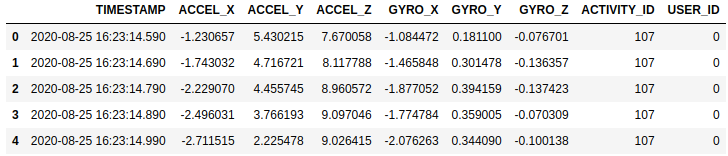
\includegraphics[width=1\textwidth, height=0.25\textheight]{Data.png}
	
	\caption{Πρώτες πέντε εγγραφές του πίνακας δεδομένων.}
	\label{plot:epoch-error}
\end{figure}
\noindent
όπου η κολόνα \en TIMESTAMP \gr αναφέρεται στο χρόνο δειγματοληψίας της εγγραφής, η κολόνα \en ACCEL\_\{X,Y,Z\} \gr αναφέρεται στην μέτρηση του επιταχυνσιομέτρου στον άξονα \{$x, y, z$\}, η κολόνα \en GYRO\_\{X,Y,Z\} \gr αναφέρεται στην μέτρηση του γυροσκοπίου στον άξονα \{$x, y, z$\}, η κολόνα \en ACTIVITY\_ID \gr δηλώνει την δραστηριότητα που πραγματοποιεί ο χρήστης και τέλος η κολόνα \en USER\_ID \gr αναφέρεται στον ποίος χρήστης έκανε την δραστηριότητα. Οι μετρήσεις των αισθητήρων καταγράφουν δείγματα στον τρισδιάστατο χώρο, αυτός είναι και ο λόγος που κάθε αισθητήρας έχει μετρήσεις τριών τυχαίων μεταβλητών ($x, y, z$). Επίσης ο κάθε χρήστης έχει μοναδικό \en ID\gr. Πλέον τα δεδομένα έχουν κατασκευαστεί και αποθηκευτεί με τέτοιο τρόπο, ώστε να είναι έτοιμα για να χρησιμοποιηθούν για το πρόβλημα της αυτόματης ταξηνόμησης ακολουθίας $\{(X_{i}, y_{i})\}_{i=1}^{N}$, με κατηγορία $y_{i}$ για κάθε ακολουθία $X_{i}$. Η κάθε ακολουθία $X_{i}$ μοντελοποιείται σαν πολυδιάστατη χρονοσειρά αισθητηριακών σημάτων, έχοντας $Τ_{i}$ δείγματα $\left<x_{1}, x_{2}, ..., x_{T_{i}}\right>$, με κατηγορία δραστηριότητας $y_{i}$. Τέλος τo κάθε δείγμα $x_{j} = [ACCEL\_X, ACCEL\_Y, ACCEL\_Z, GYRO\_X, GYRO\_Y, GYRO\_Z]$ και με $y_{j} = ACTIVITY\_ID$.

\section{Αυτόματη Kατάτμηση}
Μετά την συλλογή των δεδομένων που μοντελοποιούνται σαν πολυδιάστατη χρονοσειρά αισθητηριακών σημάτων ακολουθεί η προ-επεξεργασία τους. Το πρώτο βασικό βήμα της προ-επεξεργασίας είναι η αυτόματη κατάτμηση του σήματος. Για την επίτευξη της αυτόματης κατάτμησης έγινε χρήση της συνάρτησης \en Segment(width, overlap) \gr της βιβλιοθήκης \en seglearn \cite{arXiv:1803.08118} \gr. Η συνάρτηση λαμβάνει ως είσοδο το αρχικό σήμα και το τμηματοποιεί σε τμήματα μεγέθους \en width\gr, κάνοντας χρήση ενός επικαλυπτόμενου κυλιόμενου παραθύρου (\en sliding window\gr) σταθερού μήκος, στην περίπτωσή μας το \en width \gr ίσο με 5 δευτερόλεπτα. Με αυτήν την μέθοδο κατασκευάζουμε ένα τρισδιάστατο χρονικό τένσορα $\phi_{i} = \left<W_{1}, ..., W_{M}\right>$ και για κάθε χρονοσειρά $X_{i}$. Ο τένσορας $\phi_{i}$ έχει σχήμα $\left(M_{i}, width, 6\right)$ με $width$ το μήκος του παραθύρου και $M_{i}$ ο αριθμός των παραθύρων που κατασκευάστηκαν για κάθε χρονοσειρά $X_{i}$. Το τελικό σύνολο δεδομένων είναι το σύνολο όλων των τμημάτων που παρήχθησαν από το κυλιόμενο παράθυρο και συμβολίζεται $\{W_{i}, y_{i}\}_{i=1}^{N_{w}}$, όπου το $N_{w}$ είναι το πλήθος των τμημάτων του συνόλου δεδομένων. Το πρόβλημα μηχανικής μάθησης της ταξινόμησης των πολυδιάστατων χρονοσειρών του έργου διατυπώθηκε και αξιολογήθηκε ως ταξινόμηση του τμηματοποιημένου συνόλου δεδομένων $\{W_{i}, y_{i}\}_{i=1}^{N_{w}}$.

%\addstarredchapterc{\bibname} % minitoc
\en
\bibliographystyle{ieeetr}
\bibliography{Bibliography}

\end{document}